\chapter{Generazione delle Pseudo-Label (WSOL)}
\label{chap:wsol}

\section{Dalle Mappe di Attivazione ai Bounding Box}
\label{sec:wsol_pipeline}
Nella \textit{Weakly-Supervised Object Localization} (WSOL), l'obiettivo è ricavare le coordinate geometriche degli oggetti disponendo soltanto delle etichette a livello di immagine. Le feature estratte da DINOv3 consentono di costruire mappe di salienza continua $M \in \mathbb{R}^{H \times W}$ tramite quattro formulazioni alternative (Linear-CAM, DINO Attn, Eigen-CAM, Grad-CAM), introdotte nella Sezione~\ref{sec:arch_wsol_cenni}.

Per passare dalla mappa di calore alle coordinate del riquadro $[x_{\min}, y_{\min}, x_{\max}, y_{\max}]$, è stata implementata la sequenza mostrata nella Figura~\ref{fig:pipeline_wsol}.

\begin{figure}[htbp]
\centering
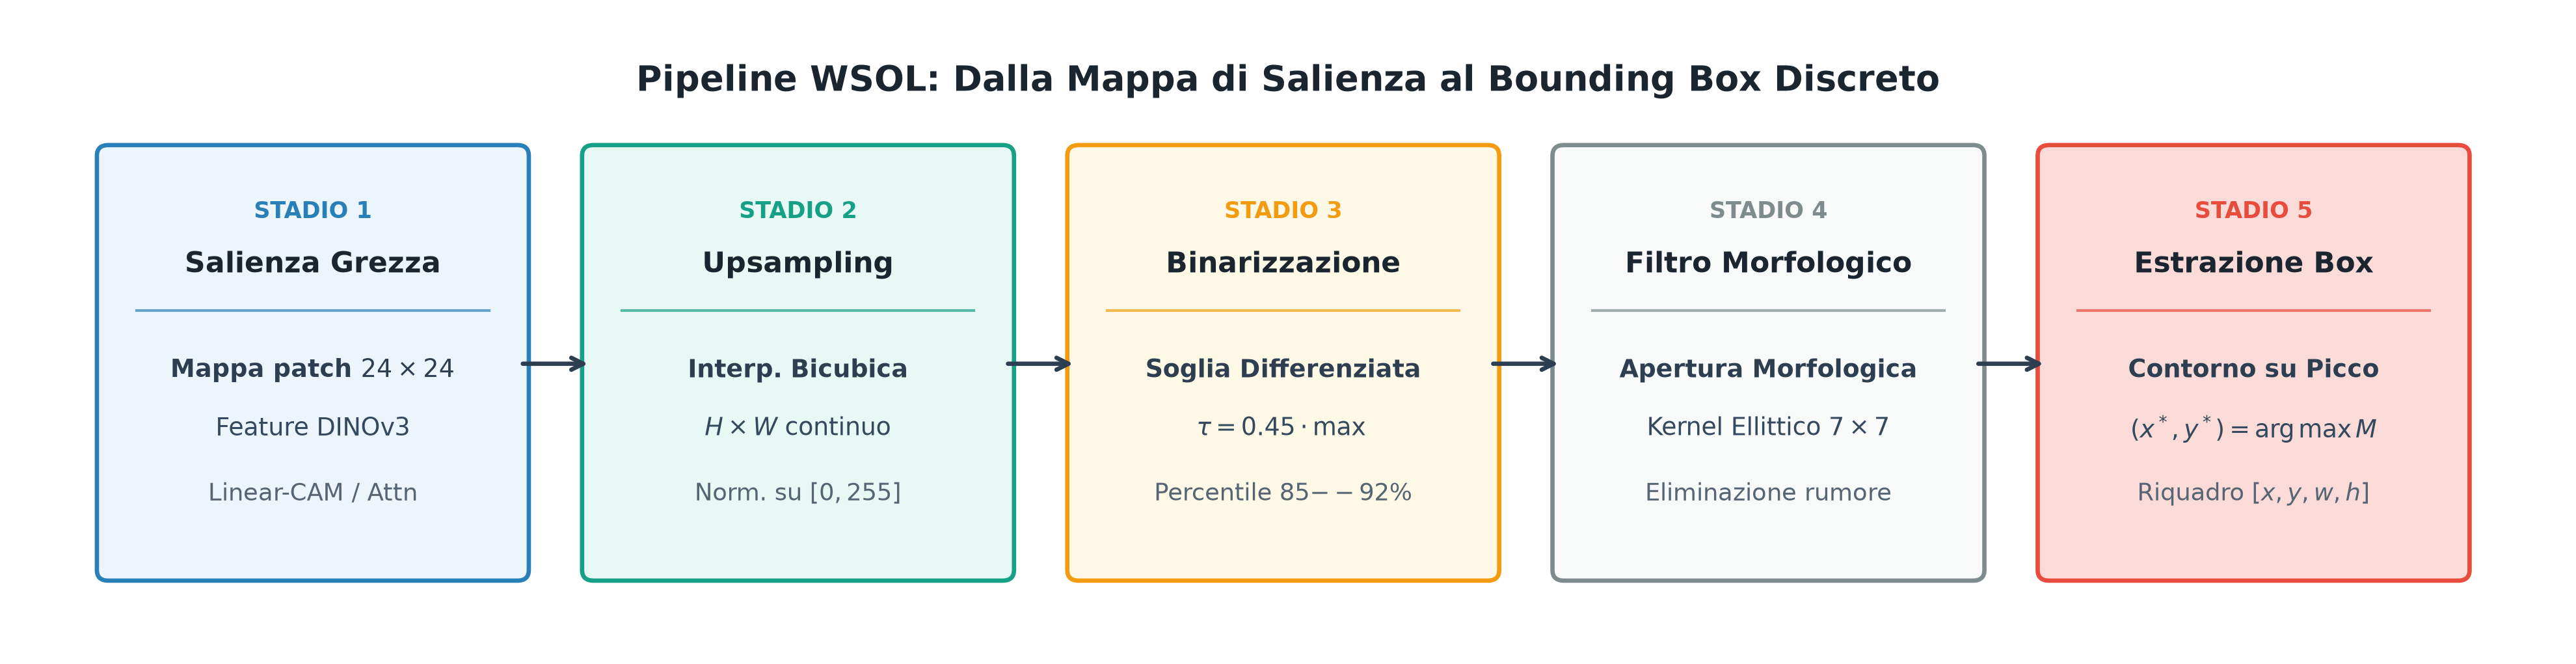
\includegraphics[width=0.92\textwidth]{figure/pipeline_wsol.png}
\caption{Pipeline di estrazione dei bounding box da mappe di salienza: normalizzazione e upsampling bicubico, binarizzazione differenziata, apertura morfologica e circoscrizione del contorno attorno al picco.}
\label{fig:pipeline_wsol}
\end{figure}

\subsection{Normalizzazione e sovracampionamento}
La mappa estratta sui token di patch $M(i, j) \in \mathbb{R}^{24 \times 24}$ viene normalizzata sull'intervallo $[0.0, 1.0]$:
\begin{equation}
    \hat{M}(i, j) = \frac{M(i, j) - \min(M)}{\max(M) - \min(M) + \epsilon}
\end{equation}
La matrice risultante viene quindi riscalata alla risoluzione originale dell'immagine $(W \times H)$ tramite interpolazione bicubica, generando una mappa di intensità $\mathcal{H}(x, y) \in [0, 255]$ a 8 bit.

\subsection{Binarizzazione differenziata}
La conversione di $\mathcal{H}(x, y)$ nella maschera binaria $B(x, y) \in \{0, 255\}$ richiede una soglia commisurata al tipo di attivazione prodotta da ciascun metodo:
\begin{itemize}
    \item \textbf{Metodi a risposta diffusa (\texttt{Linear-CAM}, \texttt{Eigen-CAM})}: le risposte coprono l'oggetto in modo omogeneo; viene applicata una soglia proporzionale al valore massimo:
    \begin{equation}
        \tau_{\text{rel}} = 0.45 \cdot \max_{x, y} \mathcal{H}(x, y)
    \end{equation}
    \item \textbf{Metodi a risposta focalizzata o sparsa (\texttt{DINO Attn}, \texttt{Grad-CAM})}: le attivazioni mostrano gradienti ripidi o picchi concentrati su pochi pixel. Una soglia proporzionale fissa porterebbe alla scomparsa della regione; viene perciò impiegata una soglia a percentile:
    \begin{equation}
        \tau_{\text{perc}} = \text{Percentile}_{85-92\%}(\mathcal{H})
    \end{equation}
    imponendo una superficie minima attiva ($A_{\min} \ge 0.05 \cdot H \cdot W$).
\end{itemize}

\subsection{Filtraggio morfologico ed estrazione del box}
Sulla maschera binaria viene applicata un'apertura morfologica con elemento strutturante ellittico $7 \times 7$:
\begin{equation}
    B_{\text{clean}} = (B \ominus K) \oplus K
\end{equation}
per eliminare il rumore isolato e ricongiungere componenti vicine.
Tra i contorni $\mathcal{C} = \{C_1, \dots, C_k\}$ individuati su $B_{\text{clean}}$, viene selezionato il poligono $C^*$ che racchiude il picco globale di salienza $(x^*, y^*) = \arg\max_{(x, y)} \mathcal{H}(x, y)$. Se nessun contorno contiene direttamente il picco, si sceglie il contorno con la maggiore intensità integrata. Il rettangolo minimo contenente $C^*$ fornisce il bounding box finale.

\section{Benchmark Comparativo sui Metodi CAM}
\label{sec:wsol_benchmark}
Per scegliere il metodo di salienza più affidabile per la successiva distillazione, è stato svolto un confronto su $57.000$ immagini di training (1.000 fotogrammi per classe). I riquadri generati sono stati confrontati con il ground truth calcolando mAP@50 (soglia IoU $\ge 0.50$) e mAP@50:95.

\section{Risultati Sperimentali e Selezione}
\label{sec:wsol_risultati}

\subsection{Confronto quantitativo globale e per Tier}
La Tabella~\ref{tab:wsol_benchmark_globale} riporta i risultati numerici dei quattro metodi sulle $57.000$ immagini, sia complessivamente sia suddivisi per tier dimensionale.

\begin{table}[htbp]
\centering
\scriptsize
\setlength{\tabcolsep}{3pt}
\begin{tabular*}{\textwidth}{@{\extracolsep{\fill}}lcccc|cccc}
\toprule
& \multicolumn{4}{c}{\textbf{Metriche Globali}} & \multicolumn{4}{c}{\textbf{mAP@50 per Tier (\%)}} \\
\textbf{Metodo CAM} & \textbf{mAP@50} & \textbf{mAP@50:95} & \textbf{Recall} & \textbf{IoU} & \textbf{Full-Fr.} & \textbf{Macro} & \textbf{Small} & \textbf{Tiny} \\
\midrule
\textbf{Linear-CAM} & \textbf{64.65\%} & \textbf{41.56\%} & \textbf{69.10\%} & \textbf{0.548} & \textbf{74.79\%} & \textbf{68.04\%} & \textbf{18.32\%} & \textbf{0.00\%} \\
\textbf{DINO Attn}  & $26.02\%$ & $16.11\%$ & $32.40\%$ & $0.312$ & $32.15\%$ & $28.40\%$ & $11.20\%$ & $0.00\%$ \\
\textbf{Grad-CAM}   & $15.70\%$ & $9.82\%$  & $21.50\%$ & $0.245$ & $19.40\%$ & $17.10\%$ & $6.40\%$  & $0.00\%$ \\
\textbf{Eigen-CAM}  & $12.94\%$ & $8.15\%$  & $17.80\%$ & $0.218$ & $16.80\%$ & $13.50\%$ & $5.10\%$  & $0.00\%$ \\
\bottomrule
\end{tabular*}
\caption{Benchmark comparativo dei metodi WSOL su $57.000$ immagini: prestazioni globali e disaggregate per scala.}
\label{tab:wsol_benchmark_globale}
\end{table}

Linear-CAM ottiene il punteggio più alto su tutte le metriche generali, superando di 38.63 punti la Self-Attention e di oltre 48 punti Grad-CAM ed Eigen-CAM. Nei tier Full-Frame e Macro raggiunge rispettivamente il $74.79\%$ e il $68.04\%$ di mAP@50, mentre si azzera sul Tier Tiny ($0.00\%$) per tutte le formulazioni.

\subsection{Analisi qualitativa e selezione}
Le differenze prestazionali riflettono la conformazione delle mappe di attivazione (Tabella~\ref{tab:comportamento_cam}).

\begin{table}[htbp]
\centering
\small
\begin{tabularx}{\textwidth}{lLL}
\toprule
\textbf{Metodo WSOL} & \textbf{Struttura dell'Attivazione} & \textbf{Rischio Principale Identificato} \\
\midrule
\textbf{Linear-CAM} & Continua, densa, guidata dai pesi di classe & Lieve dilatazione sul contesto contiguo \\
\textbf{DINO Self-Attention} & Puntiforme, focalizzata sul nucleo & Sottostima del perimetro di grandi scene \\
\textbf{Eigen-CAM} & Bimodale, guidata dal contrasto visivo & Attivazione su elementi di foreground errati \\
\textbf{Grad-CAM} & Sparsa, frammentata sulle patch & Incertezza ai bordi ad alta frequenza \\
\bottomrule
\end{tabularx}
\caption{Comportamento qualitativo e rischi strutturali dei metodi WSOL indagati.}
\label{tab:comportamento_cam}
\end{table}

Come illustrato nella Figura~\ref{fig:wsol_esempi_successo}, Linear-CAM produce una copertura uniforme e coerente con la sagoma dell'oggetto nei soggetti di scala Macro e Full-Frame (a--c), mentre manifesta dispersioni e salienze spurie sui dettagli Tiny (d--f). Per l'elevata affidabilità complessiva sui target principali, il metodo è stato selezionato per generare il dataset distillato per YOLO.

\begin{figure}[htbp]
\centering
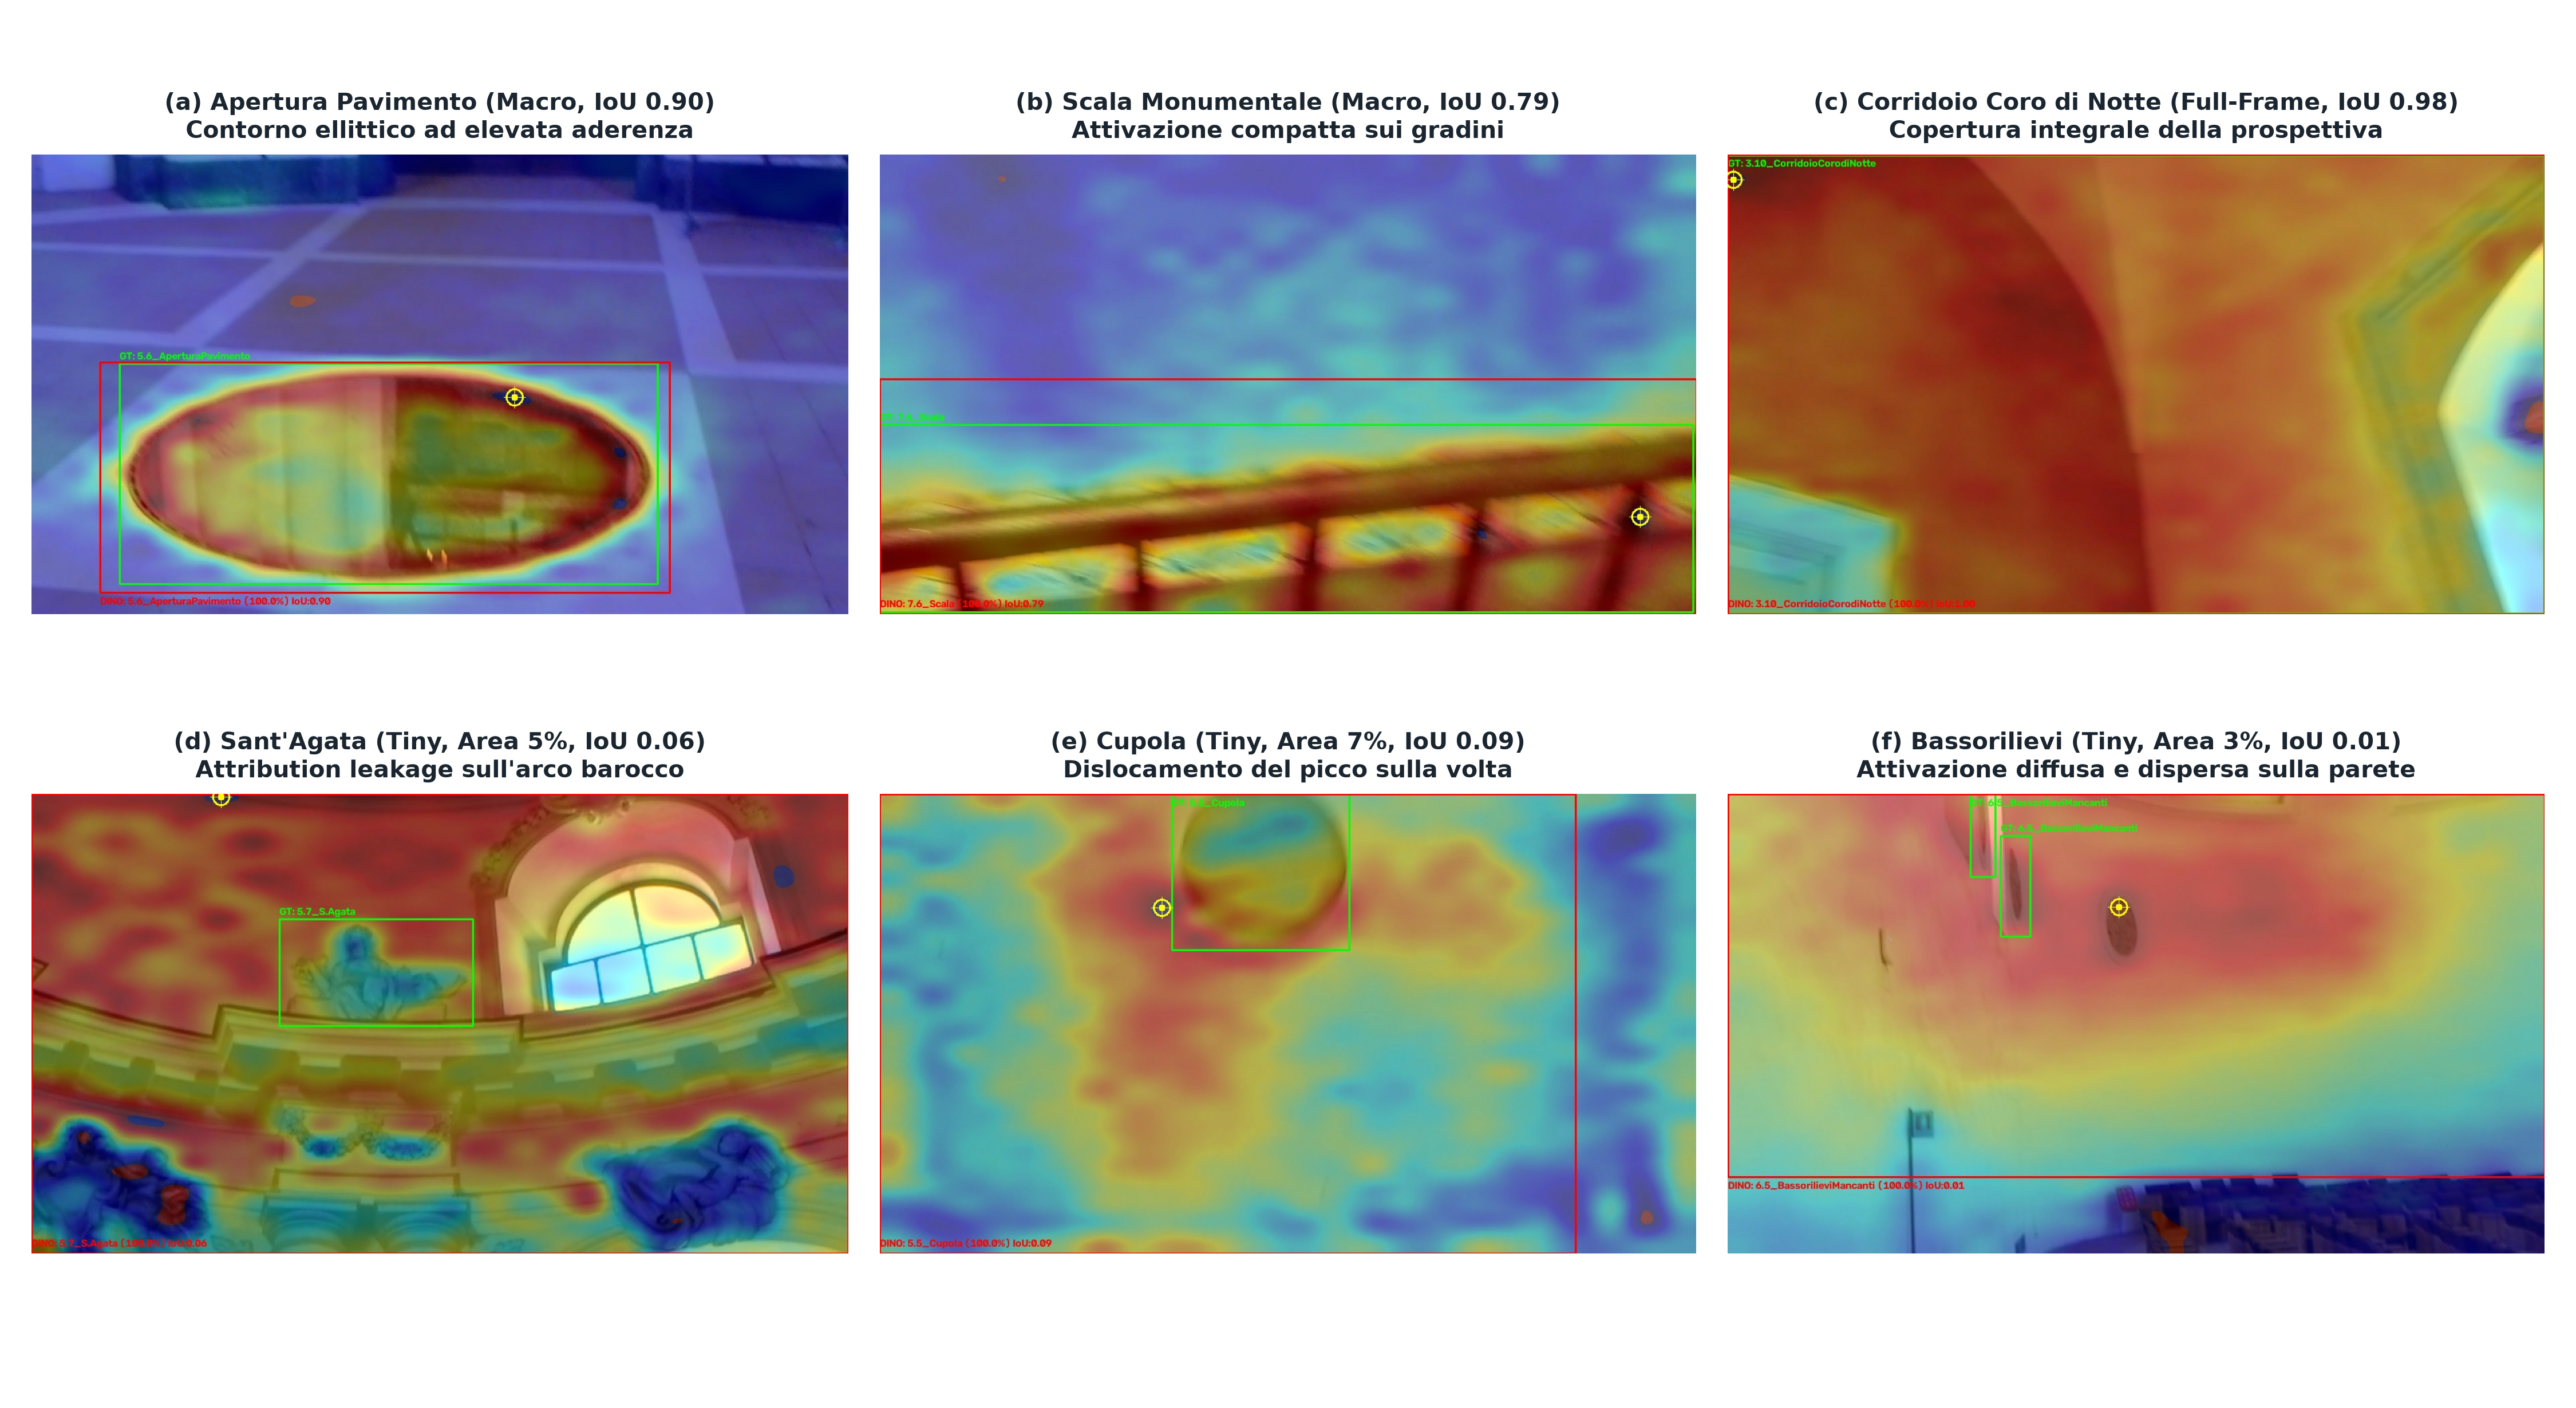
\includegraphics[width=0.88\textwidth]{figure/wsol_esempi_successo.png}
\caption{Analisi qualitativa di Linear-CAM a confronto con il ground truth: (a--c) successi su scale Macro e Full-Frame con elevata concordanza geometrica (IoU $\ge 0.79$); (d--f) fallimenti tipici su elementi Tiny dovuti a dispersione contestuale e dislocamento del picco di salienza (Verde: Ground Truth, Rosso: predizione DINO, Giallo: picco di attivazione).}
\label{fig:wsol_esempi_successo}
\end{figure}
